\documentclass{article}
\usepackage{pgfplots}
\pgfplotsset{compat=newest}

\pagestyle{empty}

\begin{document}
In this note we explore the problem of the maximum 
sub array sum in a randomly generated sequence of 
a given length.

\section{Problem statement}
The {\it Maximum Sub-array Sum} problem involves 
identifying a contiguous segment within a one-dimensional array that 
yields the highest sum. The problem is to pinpoint the subarray whose 
elements, when combined, produce the greatest total value out of all 
potential subarray combinations.

\section{Experiment setup}
To generate a sequence of length $N$ each element is independently generated
using uniform distribution of integers in the range $[-N/3, 2N/3]$. For each
$N$ we performed $200$ experiments. The blue graph below shows the maximum 
sub array sum plus-minus standard deviation using Kadane's algorithm. 
The red graph shows function 0.1667 * $x^2$ which grows almost at the same 
rate, supporting the hypothesis that average sum of maximum sub array of 
size $N$ is $O({N^2})$.

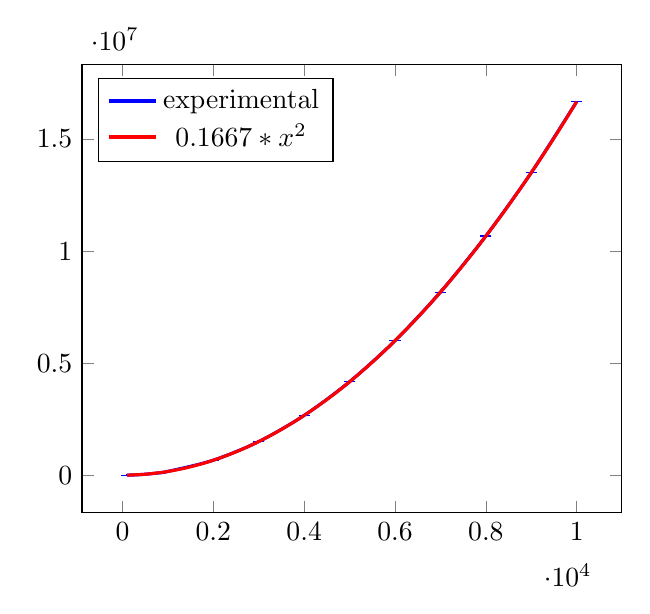
\begin{tikzpicture}
\begin{axis}[legend pos=north west]
\addplot+[line width=0.4mm,smooth,mark=,error bars/.cd, y dir=both,y explicit ]
    coordinates {
        (100, 1694.96) +- (26.9883011692103,26.9883011692103)
        (200, 6785.45) +- (54.5063069745144,54.5063069745144)
        (300, 14988.275) +- (90.3737759253203,90.3737759253203)
        (400, 26803.625) +- (129.99393976259,129.99393976259)
        (500, 41980.26) +- (141.103977264994,141.103977264994)
        (750, 93705.45) +- (222.106320261266,222.106320261266)
        (1000, 166943.15) +- (247.487105724723,247.487105724723)
        (2000, 667865.825) +- (617.761268108482,617.761268108482)
        (3000, 1499860.49) +- (833.518620007976,833.518620007976)
        (4000, 2667845.665) +- (1113.1169807235,1113.1169807235)
        (5000, 4169698.86) +- (1280.8249921047,1280.8249921047)
        (6000, 5999632.76) +- (1725.22087351156,1725.22087351156)
        (7000, 8168654.86) +- (1948.58121986229,1948.58121986229)
        (8000, 10671388.56) +- (2121.15026256982,2121.15026256982)
        (9000, 13499809.205) +- (2610.41443509934,2610.41443509934)
        (10000, 16669537.755) +- (2647.62298958424,2647.62298958424)
    };
\addlegendentryexpanded{experimental}
\addplot+[line width=0.4mm,smooth,mark=,domain=100:10000] {0.1667 * x^2)};
\addlegendentryexpanded{$0.1667 * x^2$}
\end{axis}
\end{tikzpicture}

Vatsalya Yadav
\end{document}